\documentclass{ieeeaccess}
\usepackage{cite}
\usepackage{amsmath,amssymb,amsfonts}
\usepackage{algorithmic}
\usepackage{graphicx}
\usepackage{textcomp}
\usepackage{hyperref}
\usepackage[table]{xcolor}

\usepackage{bm}
\makeatletter
\AtBeginDocument{\DeclareMathVersion{bold}
\SetSymbolFont{operators}{bold}{T1}{times}{b}{n}
\SetSymbolFont{NewLetters}{bold}{T1}{times}{b}{it}
\SetMathAlphabet{\mathrm}{bold}{T1}{times}{b}{n}
\SetMathAlphabet{\mathit}{bold}{T1}{times}{b}{it}
\SetMathAlphabet{\mathbf}{bold}{T1}{times}{b}{n}
\SetMathAlphabet{\mathtt}{bold}{OT1}{pcr}{b}{n}
\SetSymbolFont{symbols}{bold}{OMS}{cmsy}{b}{n}
\renewcommand\boldmath{\@nomath\boldmath\mathversion{bold}}}
\makeatother

\def\BibTeX{{\rm B\kern-.05em{\sc i\kern-.025em b}\kern-.08em
    T\kern-.1667em\lower.7ex\hbox{E}\kern-.125emX}}

%Your document starts from here ___________________________________________________

\graphicspath{ {./images/} }

\begin{document}
\history{Date of publication xxxx 00, 0000, date of current version xxxx 00, 0000.}
\doi{10.1109/ACCESS.2024.0429000}

\title{Refining Software Clustering: The Impact of Code Co-Changes on Architectural Reconstruction}
\author{\uppercase{Stana Adelina Diana}\authorrefmark{1} and
\uppercase{Sora Ioana}\authorrefmark{2}
}

\address[1]{Computer Science and Engineering Department
”Politehnica” University of Timisoara, Romania (e-mail: stana.adelina.diana@gmail.com)}
\address[2]{Computer Science and Engineering Department
”Politehnica” University of Timisoara, Romania (e-mail: ioana.sora@cs.upt.ro)}

\markboth
{Author \headeretal: Preparation of Papers for IEEE TRANSACTIONS and JOURNALS}
{Author \headeretal: Preparation of Papers for IEEE TRANSACTIONS and JOURNALS}

\corresp{Corresponding author: Stana Adelina Diana (e-mail: stana.adelina.diana@gmail.com).}


\begin{abstract}
Version control systems primarily offer support for tracking and managing changes in software code, but they can also provide valuable information about the managed software. Changes in multiple software entities simultaneously can imply that these entities are connected. Software entities that change at the same time (code co-changes) are treated as a distinct category of software dependencies. In some cases, these co-changes are used together with other types of dependencies, such as structural dependencies or lexical dependencies, to enhance the understanding of a software system.


This paper proposes using code co-changes in software clustering for architectural reconstruction. Structural dependencies are the most commonly used type of dependencies in software clustering for architectural reconstruction, so we will use clustering solutions obtained from structural dependencies as the baseline for our evaluations. Our approach will be applied to four open-source projects found on GitHub. For each of the projects, we will compare and evaluate the clustering obtained by using only co-changes and the clustering obtained by using co-changes combined with structural dependencies with the baseline clustering generated solely from structural dependencies.
\end{abstract}

\begin{keywords}
Architectural reconstruction, code co-changes, logical dependencies, software clustering, software dependencies, versioning system.
\end{keywords}

\titlepgskip=-21pt

\maketitle

\section{Introduction}
\label{sec:introduction}

Software systems often face a lack of documentation. Even if there was original documentation at the beginning of development, over the years it may become outdated or lost. Additionally, the original developers may leave the company, taking with them knowledge about how the software was designed. This situation challenges the teams when it comes to maintenance or modernization. In this context, recovering the system's architecture is essential. Understanding the system's architecture helps developers better evaluate and understand the nature and impact of changes they need to make. One technique to aid in reconstructing the system architecture is software clustering. Software clustering involves creating cohesive groups (modules) of software entities based on their dependencies and interactions.

Among the dependencies that can be used for software clustering are structural dependencies (relationships between entities based on code analysis), lexical dependencies (relationships based on naming conventions), and code co-changes/logical dependencies (relationships between entities extracted from the version control system), among others. Combining multiple types of dependencies, rather than relying on just one type, can be a good approach to generate better results. However, it requires fine-tuning the amount of dependencies used from each category and scaling the coefficients attached to them. Combining dependencies without considering these aspects might lead to results that are less effective than using an individual type of dependency alone.

In this paper, we assess whether using structural dependencies combined with logical dependencies can provide better results than using each type of dependency alone. The structural dependencies are used as they are extracted from static code analysis. The logical dependencies are filtered co-changes from the version control system \cite{b15}. The reason behind filtering the co-changes and not using them as they are in the versioning system is to enhance their quality and make them easier to combine with structural dependencies, as their size can outnumber the structural dependencies \cite{b1}.

To evaluate the results, we generate software clustering on four open-source projects and use two types of metrics for comparison. One of the metrics is MQ (Modularization Quality), which evaluates the modularization quality based on the interaction between the modules and does not require any additional input besides the clustering result \cite{b2}. The other is the MoJo (Move and Join) metric, a commonly used metric for evaluating the similarity between two different software clustering results \cite{b3}. For this metric, we manually generate a base of comparison for the clustering result and compare the results against this baseline.

In Section \ref{sec:related_work}, we review the related work and previous studies that used various dependencies for software clustering and their metrics for evaluation.
Section \ref{sec:workflow_implementation} details the workflow and implementation of our approach, including the extraction and filtering of dependencies, and the clustering algorithm used.
The plan and results of our experiments on four open-source projects are presented in Section \ref{sec:experiment}. Section \ref{sec:evaluation} evaluates our results by using the Modularization Quality (MQ) metric and the Move and Join (MoJo) metric. We also manually analyze some of the clustering solutions.
Finally, Section \ref{sec:conclusion} contains our conclusions and findings.

\subsection{Abbreviations and Acronyms}

The following abbreviations and acronyms are used throughout this article:

\begin{itemize}
    \item \textbf{LD}: Logical Dependencies
    \item \textbf{SD}: Structural Dependencies
    \item \textbf{MQ}: Modularization Quality Metric
    \item \textbf{MoJo}: Move and Join Metric
\end{itemize}


Logical Dependencies (LD) refer to the relationships between software entities that have been extracted and filtered from the versioning system. If these entities are not filtered, they are simply referred to as co-changes. 
Structural Dependencies (SD), on the other hand, refer to the relationships between software entities extracted from static code analysis.
Modularization Quality Metric (MQ) and Move and Join Metric (MoJo) are metrics used to evaluate software clustering results.

\section{Related Work}
\label{sec:related_work}

Software clustering for architectural reconstruction is used to place software entities in meaningful modules (clusters). Various approaches and metrics have been used to improve the quality of clustering solutions. This section presents some of the works related to the use of dependencies, clustering algorithms, and evaluation metrics.

\subsection{Dependency Types}

Software clustering relies on various types of dependencies to identify relationships between software entities. \textit{Structural dependencies}, extracted from static code analysis, have been mostly used due to their reliability \cite{b12}. However, recent research has started incorporating other types of dependencies besides structural dependencies.

Among the additional types of dependencies used in software clustering are \textit{lexical dependencies}, which can be obtained from code comments \cite{b13} or the names of source files \cite{b14}, and \textit{logical dependencies}, which are derived from co-change information in version control systems \cite{b16}.

\subsection{Clustering Algorithms}

Various clustering algorithms are used to group software entities into modules. These include hierarchical clustering for building clusters based on their hierarchical relationships \cite{b12}, \cite{b16}, K-Means clustering for partitioning entities based on their nearest mean \cite{b17}, graph-based clustering for identifying densely connected subgraphs, density-based clustering, such as DBSCAN, for grouping entities based on neighborhood density. The Louvain algorithm, which we will use in our experiments, was developed by Blondel et al., and it is a community detection algorithm commonly used for finding partitions in large networks \cite{b8}, \cite{b9}.

\subsection{Evaluation Metrics}

Evaluating the quality of clustering solutions is important for assessing the effectiveness of both the clustering algorithm and the inputs to the clustering algorithm. Mancoridis et al. introduced the Modularity Quality (MQ) metric, which evaluates the difference between connections within clusters and connections between different clusters \cite{b10}.

The Move and Join (MoJo) metric, introduced by Tzerpos et al., measures the effort required to transform one clustering solution into another through move and join operations. This metric provides a measure of similarity between the obtained clustering solution and a baseline clustering solution \cite{b11}.

\subsection{Overview}

 Table \ref{tab:related_work} provides a summary of related works that use various types of dependencies in software clustering and the algorithms applied.

\begin{table}[h]
\caption{Summary of Related Work}
\label{tab:related_work}
\centering
\setlength{\tabcolsep}{3pt}
\begin{tabular}{|l|p{2cm}|p{3cm}|}
\hline
\textbf{Paper Ref.} & \textbf{Types of Dependencies Used} & \textbf{Clustering Algorithm} \\
\hline
Corazza et al. \cite {b13} & Lexical dependencies (Code Comments) & Hierarchical Agglomerative Clustering (HAC)  \\
\hline
Anquetil et al.  \cite {b14} & Lexical dependencies (File Names, Routine Names, Included Files, Comments) & N-grams based clustering   \\
\hline
Mancoridis et al. \cite {b10}, \cite{b101} & Structural dependencies & Search based algorithm (Hill-climbing)   \\
\hline
Sora et al. \cite{b12} & Structural dependencies  & Minimum Spanning Tree based algorithms; Metric Based; Search based algorithm (Hill-climbing); Hierarchical clustering\\
\hline
Prajapati et al. \cite{b18} & Structural, Lexical, and Changed-history dependencies & Many objective optimization algorithm\\
\hline
Silva et al. \cite{b16} & Co-change dependencies & Agglomerative Hierarchical Clustering (Chameleon algorithm)\\
\hline
\end{tabular}
\end{table}




\section{Theoretical Background, Workflow, and Implementation}
\label{sec:workflow_implementation}

To achieve our goal of evaluating how the quality of clustering solutions is impacted by logical dependencies, we developed a Python tool capable of using any type of dependency, either alone or combined with other types of dependencies, as long as they are provided in CSV format. The tool clusters and evaluates software clustering solutions using either the MQ metric or the MoJo metric. In the following subsections, we present how we obtain the structural dependencies and logical dependencies used, the type of clustering algorithm we use, and the tool's workflow.

\subsection{Structural Dependencies}
\label{subsec:sd}

The structural dependencies are obtained using a tool from our previous research. While the tool primarily exports the key class ranking of a software system, it also has the capability to export the data in CSV format. The exported dependencies are directed and weighted based on the type of dependency they represent.

\Figure[t!](topskip=0pt, botskip=0pt, midskip=0pt)[width=\textwidth]{codegraph.png}
{ \textbf{Combine SD and LD.}\label{fig:codegraph}}

\subsection{Logical Dependencies}
\label{subsec:ld}

We refer to logical dependencies as the filtered co-changes between software entities. A co-change occurs when two or more software entities are modified together during the same commit in the version control system. Co-changes indicate that these entities are likely related or dependent on each other, directly or indirectly.

There is a degree of uncertainty associated with co-changes. Compared to structural dependencies, where the presence of a dependency is certain, co-changes are less reliable. For example, if the system was migrated from one version control system to another, the first commit will include all the entities from the system at that point in time. Should we consider all these entities as related to one another in this case? This would introduce false dependencies and reduce the likelihood of achieving accurate results when combining them with more reliable types of dependencies.

Even if we address the issue of the first commit, it can still happen that a developer resolves multiple unrelated issues in the same commit (even though this is not recommended by development processes).

To solve this problem, in our previous works, we refined some filtering methods to ensure that the co-changes that remain after filtering are more reliable and suitable for use with other dependencies or individually \cite{b4}, \cite{b5}, \cite{b6}. Based on our previous results, the filters we decided to use further in our research are the commit size filter and the strength filter. Both filters are used together, and the end result is the set of logical dependencies that we use to generate software clusters.

\subsubsection{Commit Size Filter}

The commit size filter filters out all co-changes that originate from commits that exceed a certain number of files.

We are interested in extracting dependencies from code commits that involve feature development or bug fixes because that is when developers change related code files. If multiple unrelated features or bug fixes are solved in a single commit, it will appear as though all the entities in those files are related, even if they are not.

One scenario where this issue arises is the first commit of a software system when it is ported from one versioning system to another. This commit will contain many changed code files, but these changes do not originate from any functionality change, so they generate numerous irrelevant co-changes for the system.

A similar scenario occurs with merge commits. A merge commit is created automatically when you perform a merge operation to integrate changes from one branch into another. After integration, all commits from the branch are added to the target branch, and on top of that, there is the merge commit containing all changes from the commits merged into a single commit. Since this commit contains only a merge of multiple smaller, related issues/features solved, it is better to gather information from the smaller commits rather than from the overall merge commit.
What both scenarios above have in common is the large number of files involved in the commits. Based on our previous research and measurements regarding the number of files involved in a commit, we chose to set a threshold of 20 files \cite{b4}, \cite{b5}. Therefore, all co-changes that originate from commits with more than 20 changed code files are filtered out.


Table \ref{tab:commit_statistics} presents the commit statistics for the studied projects. The columns represent the percentage of commits that modified under 5 files, between 5 and 10 files, between 10 and 20 files, and above 20 files. The last column indicates the average number of files changed per commit. We can observe that most of the commits have under 5 files changed, with Apache Tomcat having more than 90\% of the commits with less than 5 files changed. On the opposite side, only a few commits involve more than 20 files changed, Hibernate ORM having the highest percentage at 8.39\%. Overall, filtering based on commit size does not significantly reduce the number of commits considered.

\begin{table}[ht]
    \centering
    \caption{Commit statistics for studied projects}
    \label{tab:commit_statistics}
    \begin{tabular}{|l|c|c|c|c|c|}
        \hline
 \textbf{Project Name} & \textbf{Under 5} & \textbf{5-10} & \textbf{10-20} & \textbf{Above 20} & \textbf{Avg. Files} \\ 
        & \textbf{Files} & \textbf{Files} & \textbf{Files} & \textbf{Files} & \textbf{Changed} \\ \hline
        Apache Ant & 83.83\% & 7.50\% & 4.17\% & 4.50\% & 5.77 \\ \hline
        Apache Tomcat & 90.95\% & 5.44\% & 2.04\% & 1.58\% & 2.89 \\ \hline
        Hibernate ORM & 71.74\% & 12.37\% & 7.50\% & 8.39\% & 11.98 \\ \hline
        Gson & 83.63\% & 9.85\% & 3.70\% & 2.81\% & 4.07 \\ \hline
    \end{tabular}
\end{table}


\subsubsection{Strength Filter}

This filter focuses on the reliability of the co-changes. If a pair of co-changing entities appears only once in the entire history of the system, it might be less reliable than a pair that appears more frequently.

Zimmermann et al. introduced the support and confidence metrics to measure the significance of co-changes \cite{b7}.

The \textit{support metric} of a rule $(A \rightarrow B)$ where A is the antecedent and B is the consequent of the rule, is defined as the number of commits (transactions) in which both entities are changed together.

The \textit{confidence metric} of $(A \rightarrow B)$, as defined in Equation \eqref{eq:confidence} , focuses on the antecedent of the rule and is the number of commits together of both entities divided by the total number of commits of (A).


\begin{equation}
\text{Confidence}(A \rightarrow B) = \frac{\text{Nr. of commits containing } A \text{ and } B}{\text{Nr. of commits containing } A}
\label{eq:confidence}
\end{equation}


The confidence metric favors entities that change less and more frequently together, rather than entities that change more with a wider variation of other entities.

Assuming that (A) was changed in 10 commits and, of these 10 commits, 9 also included changes to (B), the confidence for the rule $(A \rightarrow B)$ is 0.9. On the other hand, if (C) was changed in 100 commits and, of these 100 commits, 50 also included changes to (D), the confidence for the rule $(C \rightarrow D)$ is 0.5. Therefore, in this scenario, we would have more confidence in the first pair $(A \rightarrow B)$ than in the second pair $(C \rightarrow D)$, even though the second pair has more than five times more updates together.

To favor entities that are involved in more commits together, we calculated a \textit{system factor}. This system factor is the mean value of the support metric values for all entity pairs.

The system factor is multiplied with the calculated confidence metric value. In addition, since we plan to use the metric values as weights, together with the weights of the structural dependencies, we multiply by 100 to scale the metric value to be supraunitary, and we clip the results between 0 and 100.


We refer to this addition to the original calculation formula as strength metric, and it is defined in Equation \eqref{eq:strength}.

\begin{equation}
\text{strength}(A \rightarrow B) = \text{confidence}(A \rightarrow B) \times 100 \times \text{system factor} 
\label{eq:strength}
\end{equation}


\subsubsection{Filter Application Process}

The overall filter application process is illustrated in Fig. \ref{fig:filtering}.  We begin by extracting all co-changes from the versioning system, and the first filter applied is the commit size filter. The commit size filter has a strict threshold of 20 files, meaning that any co-changes from commits involving more than 20 files are filtered out.

The co-changes that remain after applying the commit size filter are then processed using the strength filter. The strength filter uses multiple thresholds, specifically 10 different thresholds. We start with a threshold of 10 and increment it by 10 until we reach a maximum value of 100. The reason for not using a fixed threshold is to assess how different strength thresholds affect our cluster generation. 

\begin{figure}[t!]
  \centering
  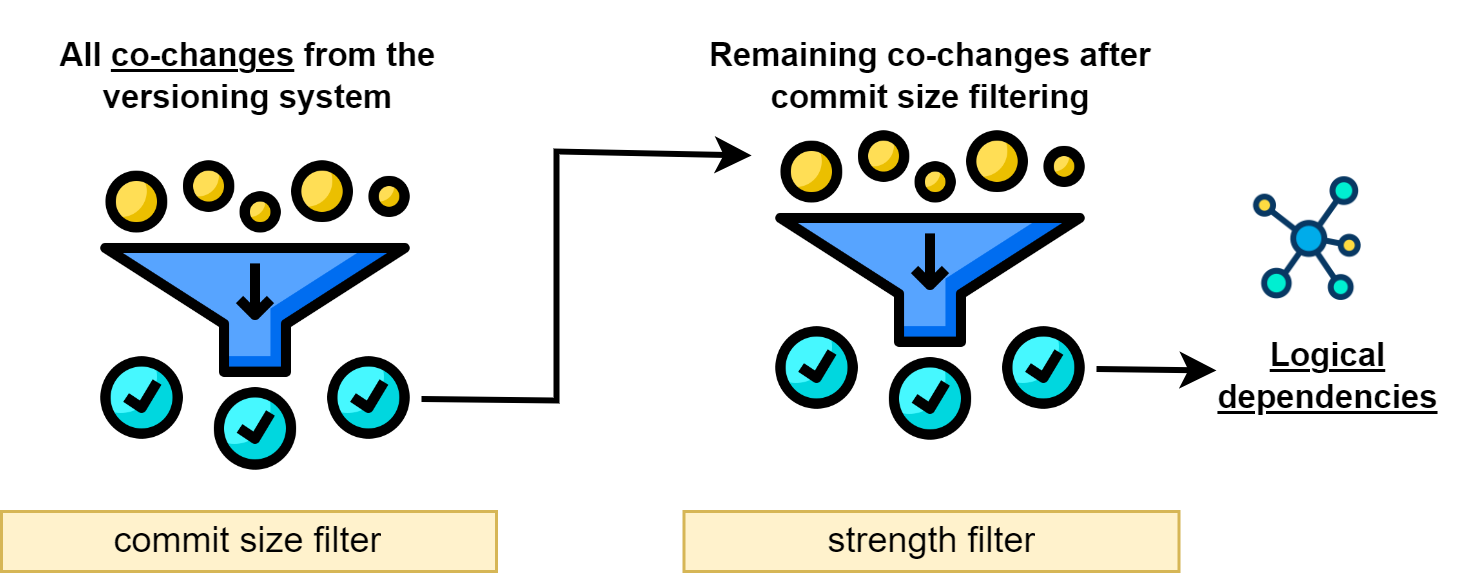
\includegraphics[width=\columnwidth]{filtering.png}
  \caption{ \textbf{Filter application process}}
  \label{fig:filtering}
\end{figure}

To extract and filter the co-changes, we used a previously developed tool \cite{b4}. This tool takes as input the GitHub repository address and the threshold values for commit and strength filters. The tool clones the repository, downloads all commit diffs starting from the first commit, examines all files changed in each commit to identify which entities have changed in those files, and creates undirected co-change dependencies between all changed entities within a commit.

The commit size filter is applied to these undirected co-change dependencies, since the metric value for $(A \rightarrow B)$ is the same as for $(B \rightarrow A)$. For the strength filter, each co-change dependency is converted into a directed co-change dependency, so for each $(A \rightarrow B)$ dependency we have both $(A \rightarrow B)$ and $(B \rightarrow A)$. This conversion is necessary because, as mentioned in the previous section, the confidence filter, upon which the strength filter is built, evaluates the antecedent of the rule. Thus, the metric value for $(A \rightarrow B)$ differs from the metric value for $(B \rightarrow A)$.

The remaining dependencies after applying the strength filter are then exported to a CSV file for further use.

\Figure[t!](topskip=0pt, botskip=0pt, midskip=0pt)[width=\textwidth]{workflow-tool.png}
{ \textbf{Tool workflow overview: input, processing and output.}\label{fig:tool}}

\subsection{Louvain Clustering Algorithm}
\label{subsec:louvain}

The Louvain algorithm was originally developed by Blondel et al. and is used for finding community partitions (clusters) in large networks. The algorithm begins with a weighted network of N nodes, initially assigning each node to its own cluster, resulting in N clusters. For each node, the algorithm evaluates the modularity gain from moving the node to the cluster of each of its neighbors. Based on the results, the node is moved to the cluster with the maximum positive modularity gain. This process is repeated for all nodes until no further improvement in modularity is possible \cite{b8}.

The modularity of a cluster is a value that ranges from -1 to 1, which measures the density of connections inside clusters compared to connections between clusters \cite{b9}.

\subsection{Clustering Result Evaluation}
\label{subsec:evaluation_def}

To evaluate the clustering results, we use two metrics: the Modularity Quality (MQ) metric and the Move and Join (MoJo) metric. Each of these metrics provides a different perspective on the quality of the clustering solutions. Both metrics are integrated into our tool and receive as input the generated clustering solution.

\subsubsection{Modularity Quality Metric}

Mancoridis et al. introduced the Modularity Quality (MQ) metric to evaluate the modularization quality of a clustering solution based on the interaction between modules (clusters) \cite{b2},\cite{b10}. It evaluates the difference between connections within clusters and connections between different clusters.

The MQ of a graph partitioned into \( k \) clusters, where \( A_i \) is the Intra-Connectivity of the \( i \)-th cluster and \( E_{ij} \) is the Inter-Connectivity between the \( i \)-th and \( j \)-th clusters, is calculated using Equation \eqref{eq:mq} \cite{b2}.

\begin{equation}
MQ = \left( \frac{1}{k} \sum_{i=1}^{k} A_i \right) - \left( \frac{1}{k(k-1)} \sum_{i,j=1}^{k} E_{ij} \right)
\label{eq:mq}
\end{equation}

The MQ metric outputs a value between -1 and 1, where -1 indicates that there is no cohesion between the clusters of the clustering solution, and 1 indicates that there is no coupling between them.

The MQ metric is useful because it does not require any additional input besides the clustering result itself. It relies on the structure of the clustered entities and their interactions. 

\subsubsection{MoJo Metric}

The Move and Join (MoJo) metric was introduced by Tzerpos et al. to evaluate the similarity between two different software clustering results. The metric measures the effort required to transform one clustering solution into another through move and join operations \cite{b3}, \cite{b11}.

To use the MoJo metric, we first generate a baseline clustering solution for comparison. This baseline is manually created based on our analysis of the code base. The MoJo metric then calculates the minimal number of move and join operations needed to convert the generated clustering solution into the baseline clustering solution.

The formula for the MoJo metric is represented in Equation \eqref{eq:mojo}, where \( \text{mnr}(A, B) \) is the minimum number of operations to transform cluster \( A \) into cluster \( B \) and \( \text{mnr}(B, A) \) is the minimum number of operations to transform cluster \( B \) into cluster \( A \) \cite{b3}. 


\begin{equation}
\text{MoJo}(A, B) = \min(\text{mnr}(A, B), \text{mnr}(B, A))
\label{eq:mojo}
\end{equation}

By using the MoJo metric, we can evaluate the similarity between the generated clustering solutions and the expected clustering structure. We consider this metric useful when combining multiple types of dependencies because it clearly measures the similarity between the obtained clustering solutions and the same baseline.

\subsection{Tool Workflow Overview}
\label{subsec:tool_workflow}

To generate the cluster solutions and evaluate the results, we created a tool in Python. The entire workflow of the tool is presented in Fig. \ref{fig:tool}.

\subsubsection{Input}

The tool takes as input one or multiple dependency CSV files and the baseline solution required for the MoJo metric. We designed the tool to accept multiple dependency files so that we can generate clustering solutions based on either a single type of dependency (structural or logical) or a combination of both.

Since the MoJo metric requires a baseline solution to evaluate the generated solution, we manually inspected the code and created baseline clustering solutions, which we then provide as input for the tool.

\subsubsection{Processing}

The dependencies are saved in the CSV file in the following format: antecedent of a dependency, consequent of a dependency, weight. The tool reads each line, adds the antecedent and consequent as nodes in a directed graph, and creates an edge between them, with the weight from the CSV file becoming the edge weight. If multiple dependency files are processed and the same dependency is found in multiple files, the edge weights are summed.


After all dependencies are read, the directed graph is passed to the Louvain clustering algorithm to generate the clustering result. The clustering result is then evaluated. The MQ metric requires the directed graph and the clustering result, while the MoJo metric requires the baseline clustering solution provided as input and the clustering result.

\subsubsection{Output}

After both evaluations are done, we export the clustering result, the cluster count, and the values for both metrics.

\section{Experimental Plan and Results}
\label{sec:experiment}

\begin{figure}[t!]
  \centering
  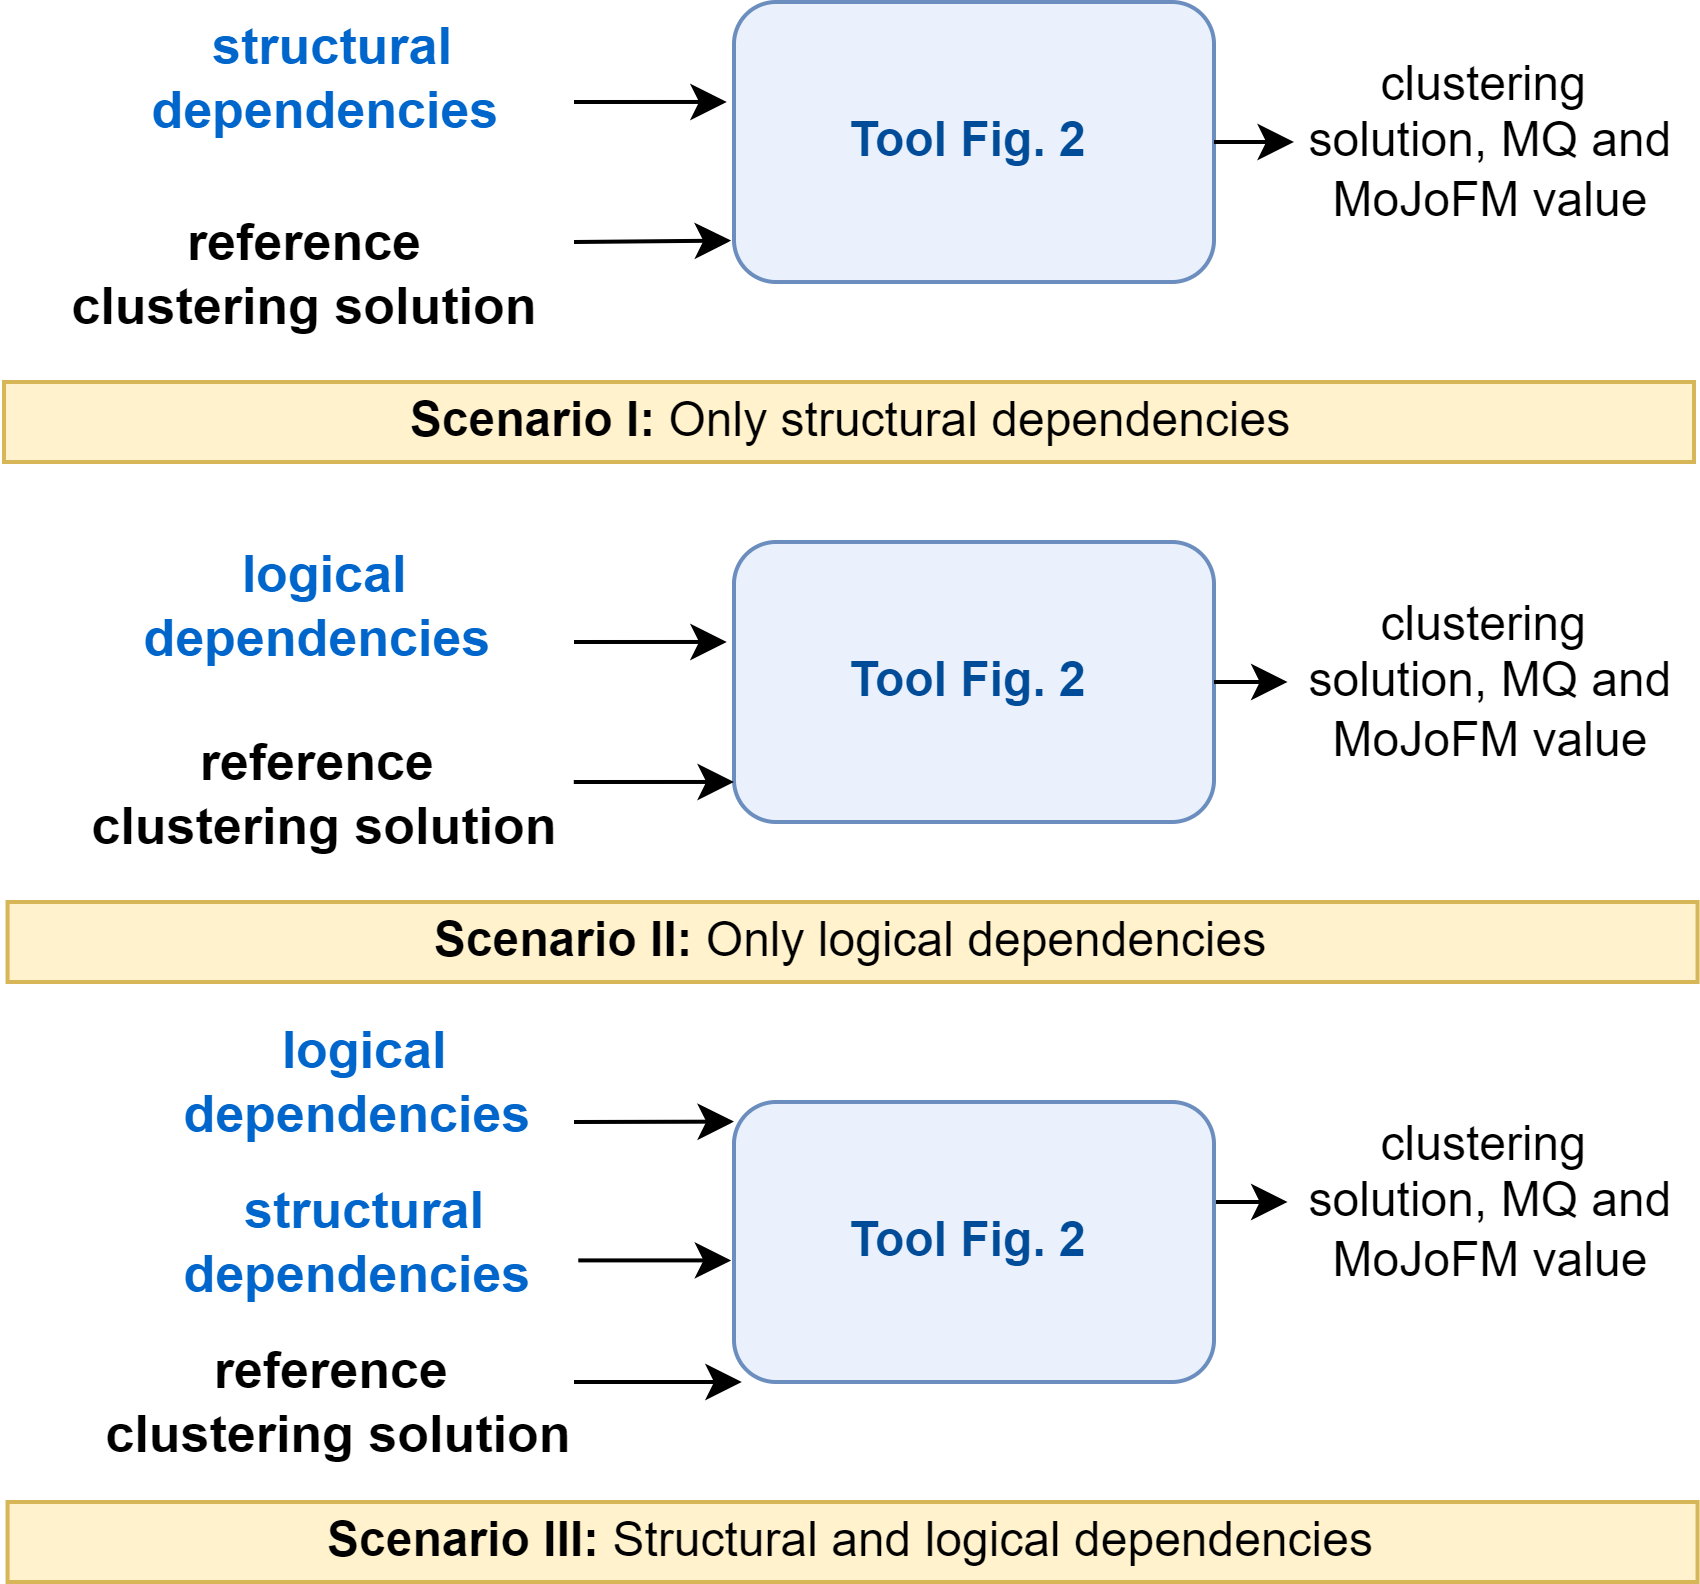
\includegraphics[width=\columnwidth]{scenario.png}
  \caption{ \textbf{Scenarios for results}}
  \label{fig:scenatrio}
\end{figure}

\begin{table*}
\centering
\caption{Overview of projects used in experimental analysis}
\label{tab:project_info}
\setlength{\tabcolsep}{7pt} 
\begin{tabular}{|l|l|c|l|p{4cm}|}
\hline
\textbf{Project Name} & \textbf{Release Tag} & \textbf{Number of Commits} & \textbf{GitHub Repository Link} & \textbf{Repository Description} \\ \hline
Apache Ant & \href{https://github.com/apache/ant/tree/rel/1.10.13}{rel/1.10.13} & 14917 & \href{https://github.com/apache/ant}{https://github.com/apache/ant} & Apache Ant is a Java-based build tool. \\ \hline
Apache Tomcat & \href{https://github.com/apache/tomcat/tree/8.5.93}{8.5.93} & 22698 & \href{https://github.com/apache/tomcat}{https://github.com/apache/tomcat} & Apache Tomcat software powers numerous large-scale, mission-critical web applications across a diverse range of industries and organizations. \\ \hline
Hibernate ORM & \href{https://github.com/hibernate/hibernate-orm/tree/6.2.14}{6.2.14} & 16609 & \href{https://github.com/hibernate/hibernate-orm}{https://github.com/hibernate/hibernate-orm} & Hibernate ORM is a powerful object/relational mapping solution for Java. \\ \hline
Gson & \href{https://github.com/google/gson/tree/gson-parent-2.10.1}{gson-parent-2.10.1} & 1772 & \href{https://github.com/google/gson}{https://github.com/google/gson} & A Java serialization/deserialization library to convert Java Objects into JSON and back. \\ \hline
\end{tabular}
\end{table*}

\subsection{Experimental Plan}
\label{subsec:plan}

\subsubsection{Tool Runs}
The objective of our research is to evaluate how the quality of software clustering solutions is impacted by logical dependencies.
To assess the impact, we run the tool presented in Section \ref{subsec:tool_workflow} in three different scenarios. All three scenarios are illustrated in Fig. \ref{fig:scenatrio}.

In the first scenario, we run the tool once, providing only the structural dependencies of the system as input for the clustering algorithm.

In the second scenario, we run the tool ten times, using only logical dependencies as input. We perform ten runs because we generate logical dependencies with different threshold values for the strength filter. We start with a threshold of 10 and increase it in steps of 10 up to 100, where 100 is the maximum value for the threshold.

In the third scenario, we combine logical with structural dependencies. Again, we run the tool ten times, each time using structural dependencies and logical dependencies generated with different strength thresholds.




\subsection{Results}
\label{subsec:results}

\subsubsection{Overview of projects used}


In Table \ref{tab:project_info}, we have synthesized all the information about the four projects used in our experiments. The 'Project Name' column contains the names of the software projects sourced from GitHub. The 'Release Tag' column contains the specific release tag of the project that was analyzed. For logical dependency extraction, we processed all the commits starting from the first commit up to the commit associated with the specified tag. For structural dependencies, we extracted the dependencies from the code of that specific tag. The 'Number of Commits' column provides the total number of commits used for logical dependencies extraction. The 'GitHub Repository Link' column includes the URL link to the project's repository on GitHub. Finally, the 'Repository Description' column offers a brief description of the project's purpose and functionality.


We mostly chose projects with more than 10,000 commits in their commit history, so that the logical dependencies extraction can be done on a larger information base. However, we selected 'Gson', which has a relatively small commit history (1,772 commits), to determine if our experiments work with a smaller information base.

\subsubsection{Detailed Results}

\begin{table}
\caption{Clustering results based on different dependency types and strength filter thresholds for repository: \url{https://github.com/apache/ant}}
\label{tab:clustering_results_ant}
\centering
\setlength{\tabcolsep}{3pt}
\begin{tabular}{|l|c|c|c|c|c|c|}
\hline
\textbf{Dependency Type} & \textbf{Nr. of} & \textbf{Entities} & \textbf{System} & \textbf{MQ} & \textbf{MoJo} \\
\textbf{[strength thresh.]} & \textbf{clusters} & \textbf{Count} & \textbf{Cover (\%)} &  &  \\
\hline
SD & 14 & 517 & 100.00 & 0.081 & 203 \\
\hline
LD [10] & 56 & 320 & 61.90 & 0.506 & 89 \\
LD [20] & 53 & 215 & 41.59 & 0.547 & 60 \\
LD [30] & 44 & 174 & 33.66 & 0.558 & 47 \\
LD [40] & 40 & 152 & 29.40 & 0.580 & 41 \\
LD [50] & 35 & 138 & 26.69 & 0.604 & 33 \\
LD [60] & 34 & 120 & 23.21 & 0.587 & 32 \\
LD [70] & 32 & 106 & 20.50 & 0.577 & 27 \\
LD [80] & 29 & 92 & 17.79 & 0.576 & 25 \\
LD [90] & 24 & 79 & 15.28 & 0.606 & 20 \\
LD [100] & 19 & 64 & 12.38 & 0.611 & 15 \\
\hline
SD+LD [10] & 15 & 517 & 100.00 & \cellcolor[HTML]{C0C0C0}\textbf{0.144} & \cellcolor[HTML]{C0C0C0}\textbf{178} \\
SD+LD [20] & 13 & 517 & 100.00 & 0.116 & 215 \\
SD+LD [30] & 14 & 517 & 100.00 & 0.126 & 207 \\
SD+LD [40] & 14 & 517 & 100.00 & 0.124 & 208 \\
SD+LD [50] & 14 & 517 & 100.00 & 0.121 & 210 \\
SD+LD [60] & 16 & 517 & 100.00 & 0.124 & 187 \\
SD+LD [70] & 14 & 517 & 100.00 & 0.115 & 210 \\
SD+LD [80] & 14 & 517 & 100.00 & 0.115 & 210 \\
SD+LD [90] & 14 & 517 & 100.00 & 0.114 & 210 \\
SD+LD [100] & 13 & 517 & 100.00 & 0.103 & 205 \\
\hline
\end{tabular}
\end{table}

\begin{table}
\caption{Clustering results based on different dependency types and strength filter thresholds for repository: \href{https://github.com/apache/tomcat}{https://github.com/apache/tomcat}}
\label{tab:clustering_results_tomcat}
\centering
\setlength{\tabcolsep}{3pt}
\begin{tabular}{|l|c|c|c|c|c|c|}
\hline
\textbf{Dependency Type} & \textbf{Nr. of} & \textbf{Entities} & \textbf{System} & \textbf{MQ} & \textbf{MoJo} \\
\textbf{[strength thresh.]} & \textbf{clusters} & \textbf{Count} & \textbf{Cover (\%)} &  &  \\
\hline
SD & 31 & 662 & 100.00 & 0.184 & 95 \\
\hline
LD [10] & 42 & 406 & 61.33 & 0.505 & 61 \\
LD [20] & 45 & 303 & 45.77 & 0.538 & 59 \\
LD [30] & 46 & 249 & 37.61 & 0.532 & 47 \\
LD [40] & 42 & 208 & 31.42 & 0.590 & 40 \\
LD [50] & 44 & 198 & 29.91 & 0.604 & 40 \\
LD [60] & 45 & 177 & 26.74 & 0.601 & 41 \\
LD [70] & 45 & 164 & 24.77 & 0.598 & 38 \\
LD [80] & 36 & 127 & 19.18 & 0.618 & 30 \\
LD [90] & 32 & 116 & 17.52 & 0.623 & 24 \\
LD [100] & 30 & 110 & 16.62 & 0.640 & 21 \\
\hline
SD+LD [10] & 27 & 662 & 100.00 & 0.255 &  \cellcolor[HTML]{C0C0C0}\textbf{71} \\
SD+LD [20] & 28 & 662 & 100.00 &  \cellcolor[HTML]{C0C0C0}\textbf{0.265} & 81 \\
SD+LD [30] & 28 & 662 & 100.00 & 0.253 & 88 \\
SD+LD [40] & 28 & 662 & 100.00 & 0.243 & 89 \\
SD+LD [50] & 30 & 662 & 100.00 & 0.248 & 91 \\
SD+LD [60] & 30 & 662 & 100.00 & 0.237 & 87 \\
SD+LD [70] & 27 & 662 & 100.00 & 0.232 & 92 \\
SD+LD [80] & 30 & 662 & 100.00 & 0.225 & 95 \\
SD+LD [90] & 30 & 662 & 100.00 & 0.222 & 90 \\
SD+LD [100] & 30 & 662 & 100.00 & 0.222 & 90 \\
\hline
\end{tabular}
\end{table}

\begin{table}
\caption{Clustering results based on different dependency types and strength filter thresholds for repository: \href{https://github.com/hibernate/hibernate-orm}{https://github.com/hibernate/hibernate-orm}}
\label{tab:clustering_results_hibernate}
\centering
\setlength{\tabcolsep}{3pt}
\begin{tabular}{|l|c|c|c|c|c|c|}
\hline
\textbf{Dependency Type} & \textbf{Nr. of} & \textbf{Entities} & \textbf{System} & \textbf{MQ} & \textbf{MoJo} \\
\textbf{[strength thresh.]} & \textbf{clusters} & \textbf{Count} & \textbf{Cover (\%)} &  &  \\
\hline
\textbf{SD} & \textbf{26} & \textbf{4414} & \textbf{0.073} & \textbf{2668} \\
\hline
SD & 26 & 4414 & 100.00 & 0.073 & 1963 \\
\hline
LD [10] & 47 & 1450 & 32.85 & 0.414 & 674 \\
LD [20] & 64 & 1325 & 30.02 & 0.399 & 551 \\
LD [30] & 66 & 1222 & 27.68 & 0.374 & 483 \\
LD [40] & 86 & 915 & 20.73 & 0.414 & 350 \\
LD [50] & 88 & 900 & 20.39 & 0.401 & 358 \\
LD [60] & 87 & 848 & 19.21 & 0.402 & 334 \\
LD [70] & 90 & 459 & 10.40 & 0.512 & 148 \\
LD [80] & 92 & 450 & 10.19 & 0.502 & 150 \\
LD [90] & 93 & 432 & 9.79 & 0.488 & 146 \\
LD [100] & 81 & 356 & 8.07 & 0.524 & 123 \\
\hline
SD+LD [10] & 27 & 4414 & 100.00 & 0.124 &  \cellcolor[HTML]{C0C0C0}\textbf{1842} \\
SD+LD [20] & 28 & 4414 & 100.00 & 0.144 & 1868 \\
SD+LD [30] & 28 & 4414 & 100.00 &  \cellcolor[HTML]{C0C0C0}\textbf{0.149}& 1870 \\
SD+LD [40] & 30 & 4414 & 100.00 & 0.131 & 1859 \\
SD+LD [50] & 31 & 4414 & 100.00 & 0.140 & 1913 \\
SD+LD [60] & 31 & 4414 & 100.00 & 0.113 & 1913 \\
SD+LD [70] & 30 & 4414 & 100.00 & 0.105 & 1917 \\
SD+LD [80] & 28 & 4414 & 100.00 & 0.093 & 1924 \\
SD+LD [90] & 28 & 4414 & 100.00 & 0.093 & 1924 \\
SD+LD [100] & 28 & 4414 & 100.00 & 0.067 & 1924 \\
\hline
\end{tabular}
\end{table}


\begin{table}
\caption{Clustering results based on different dependency types and strength filter thresholds for repository: \href{https://github.com/google/gson}{https://github.com/google/gson}}
\label{tab:clustering_results_gson}
\centering
\setlength{\tabcolsep}{3pt}
\begin{tabular}{|l|c|c|c|c|c|c|}
\hline
\textbf{Dependency Type} & \textbf{Nr. of} & \textbf{Entities} & \textbf{System} & \textbf{MQ} & \textbf{MoJo} \\
\textbf{[strength thresh.]} & \textbf{clusters} & \textbf{Count} & \textbf{Cover (\%)} &  &  \\
\hline
SD & 10 & 210 & 100.00 & 0.139 & 44 \\
\hline
LD [10] & 10 & 66 & 31.43 & 0.571 & 27 \\
LD [20] & 11 & 50 & 23.81 & 0.547 & 16 \\
LD [30] & 12 & 41 & 19.52 & 0.544 & 10 \\
LD [40] & 8 & 31 & 14.76 & 0.635 & 5 \\
LD [50] & 8 & 31 & 14.76 & 0.600 & 5 \\
LD [60] & 8 & 28 & 13.33 & 0.552 & 6 \\
LD [70] & 7 & 26 & 12.38 & 0.579 & 5 \\
LD [80] & 5 & 18 & 8.57 & 0.590 & 3 \\
LD [90] & 5 & 18 & 8.57 & 0.590 & 3 \\
LD [100] & 5 & 18 & 8.57 & 0.590 & 3 \\
\hline
SD+LD [10] & 11 & 210 & 100.00 & \cellcolor[HTML]{C0C0C0}\textbf{0.215} & \cellcolor[HTML]{C0C0C0}\textbf{21} \\
SD+LD [20] & 10 & 210 & 100.00 & 0.182 & 22 \\
SD+LD [30] & 10 & 210 & 100.00 & 0.165 & 22 \\
SD+LD [40] & 10 & 210 & 100.00 & 0.165 & 22 \\
SD+LD [50] & 10 & 210 & 100.00 & 0.165 & 22 \\
SD+LD [60] & 10 & 210 & 100.00 & 0.164 & 22 \\
SD+LD [70] & 10 & 210 & 100.00 & 0.164 & 22 \\
SD+LD [80] & 11 & 210 & 100.00 & 0.188 & 42 \\
SD+LD [90] & 11 & 210 & 100.00 & 0.188 & 42 \\
SD+LD [100] & 11 & 210 & 100.00 & 0.188 & 42 \\
\hline
\end{tabular}
\end{table}



We present the clustering results based on different dependency types and strength filter thresholds in four tables, each corresponding to a different project. These tables provide an overview of the clustering results, underlining how various dependency types impact the clustering results. Table \ref{tab:clustering_results_ant} shows the results for Apache Ant, Table \ref{tab:clustering_results_tomcat} presents the results for Apache Tomcat, Table \ref{tab:clustering_results_hibernate} presents the results for Hibernate ORM, and Table \ref{tab:clustering_results_gson} presents the results for Gson.

Each table includes the following columns:
\begin{itemize}
\item \textbf{Dependency Type:} The type of dependency used in the clustering (SD - Structural Dependencies, LD - Logical Dependencies with various strength thresholds, and combined SD+LD).
\item \textbf{Nr. of Clusters:} The number of clusters from the clustering solution obtained.
\item \textbf{Entities Count:} The total number of software entities (such as classes, interfaces, enums) involved in clustering.
\item \textbf{System Cover:} Considering that the total number of entities extracted from the code base is the maximum number of entities in the system (first line of each table), we calculated the percentage of entities contained in the other inputs relative to the number of entities from the code base.
\item \textbf{MQ (Modularization Quality):} The result obtained when applying the MQ evaluation metric to the clustering solution.
\item \textbf{MoJo:} The result obtained when applying the MoJo evaluation metric to the clustering solution.
\end{itemize}

The rows in each table represent different dependency types and strength filter thresholds used in the clustering experiments.


\section{Evaluation}
\label{sec:evaluation}

In evaluating the clustering results, we use two metrics: MoJo and MQ. The MoJo metric measures how close the generated clustering solution is to our manually generated clustering solution. A smaller MoJo value indicates that fewer move and join operations are required to transform the generated clusters into the expected clusters.

The MQ metric's value ranges between -1 and 1. A value of -1 means that the clusters have more connections between the clusters than within the clusters, while a value of 1 means that there are more connections within clusters than between clusters. A good clustering solution should have an MQ value close to 1, since this indicates that the clusters are more cohesive internally and have fewer connections to other clusters.

The overall analysis of all the results from subsection \ref{subsec:results} indicates that combining structural and logical dependencies (SD+LD) provides better clustering solutions than using structural dependencies (SD) alone, with 100\% coverage of the system, meaning that no entity is missed during cluster generation. On the other hand, logical dependencies (LD) alone result in better clustering quality metrics compared to both SD and SD+LD, but they do not cover the entire system.

The best results for SD+LD are observed with a strength threshold between 10-30\%. For LD only, the best results are obtained at a 100\% strength threshold. The overall trend shows that for LD only, the MQ metric increases in value with a higher strength threshold, indicating more cohesive clusters, while the MoJo metric decreases, indicating that fewer transformations are needed to reach the expected clustering. For SD+LD, the best MQ and MoJo values are obtained at lower strength thresholds, and then both metrics indicate less effective clustering solution obtained with higher strength thresholds.

In the sections below, we analyze each project in detail.

\subsection{Analysis of clustering results}

\subsubsection{Apache Ant}

The clustering results for Apache Ant (Table \ref{tab:clustering_results_ant}) show that the combined structural and logical dependencies (SD+LD) achieved the best values with a strength threshold of 10, resulting in an MQ of 0.144 and a MoJo of 178.

Compared with the SD only results, where we have an MQ of 0.081 and a MoJo of 203, all SD+LD clustering solutions have better MQ metric. The MoJo metric is not always better than the SD MoJo, but the values obtained are close to the SD result.

Logical dependencies (LD) alone produced the highest MQ value (MQ = 0.611) and the lowest MoJo value (MoJo = 15) at the 100\% strength threshold, but the percentage of entities covered is significantly lower (LD[100] covers only 12.38\% of the system). On the other hand, even at the LD 10\% strength threshold (LD[10] covers only 61.9\% of the system), both metrics are performing better than SD only or SD+LD[10].

An interesting observation is that, based on the LD-only results, where the metric results improve with a higher strength threshold, the SD+LD results do not follow the same pattern. On the contrary, the SD+LD metric results decline with a higher strength threshold. The explanation for this behavior may lie in the overlap between structural and logical dependencies. As presented in Figure \ref{fig:ant_correlation}, the overlap between structural and logical dependencies might influence the clustering outcomes differently when combined than when applied separately.

\begin{figure}[t!]
  \centering
  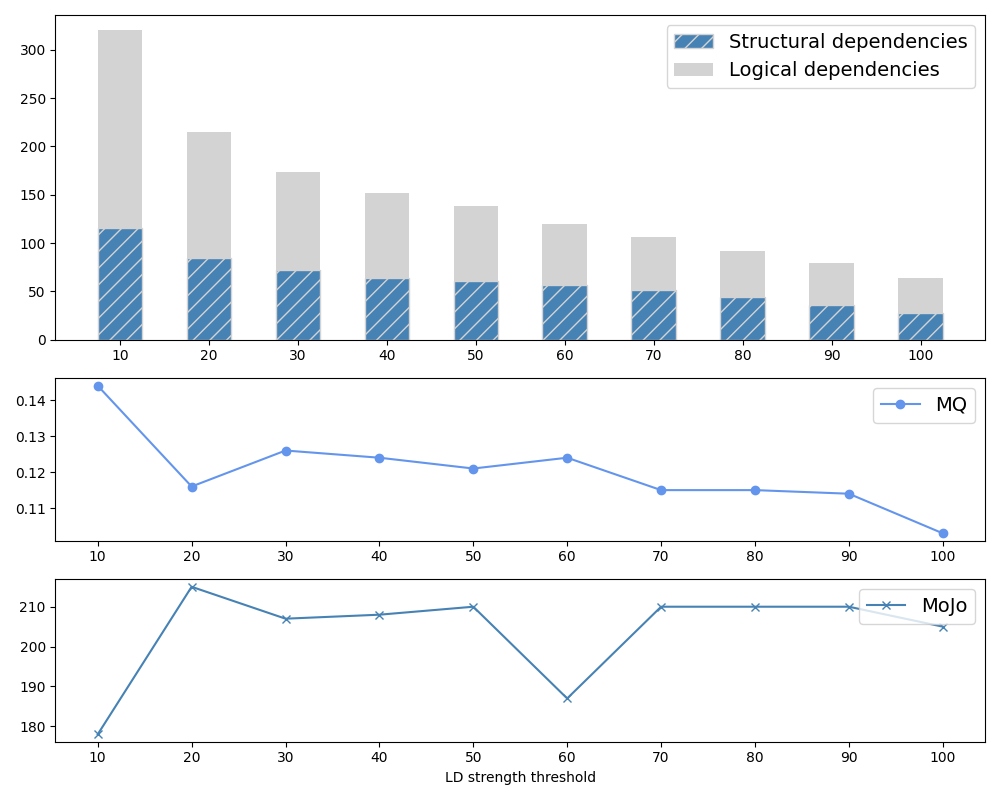
\includegraphics[width=\columnwidth]{ant_correlation.png}
  \caption{\textbf{Apache Ant: Overlap between structural and logical dependencies and its correlation with clustering metrics.}}
  \label{fig:ant_correlation}
\end{figure}

In our previous works (\cite{b4}, \cite{b5}), we studied how these two types of dependencies overlap. The reason behind this study was to check how much new information we can get from using logical dependencies and how much is already present via structural dependencies.

Our overall findings were that with stricter filtering of logical dependencies, we obtain a higher percentage of overlap between the two dependencies, reaching at most 50\% of logical dependencies that are also structural dependencies.

So, we believe that the reason why SD+LD clustering solutions decline in performance with a higher strength threshold is that there is less and less new additional information being added to the system (logical dependencies that are not structural dependencies), causing the clustering solution to start resembling the performance of the SD-only solution. This redundancy between logical and structural dependencies might not introduce new meaningful information to the clustering algorithm and can instead introduce noise.


\subsubsection{Apache Tomcat}

For Apache Tomcat (Table \ref{tab:clustering_results_tomcat}), the SD+LD[20] combination achieved the best results for the MQ metric (MQ = 0.265), while SD+LD[10] achieved the best value for MoJo (MoJo = 71).

In comparison with Apache Ant, where both metrics reached their best value at the same strength threshold, there is a difference of one strength step between the metrics' best results for Apache Tomcat. Even so, the MoJo metric for SD+LD[10] and SD+LD[20] indicates that fewer transformations are required compared to SD-only or other SD+LD combinations.

The LD-only lines show the best MQ and MoJo values for LD[100], with an MQ of 0.640 and a MoJo of 21, but coverage remains an issue, as LD[100] covers only 16.62\% of the system. On the other hand, LD[10] covers 61.33\% of the system and still provides better clustering solutions according to the MQ and MoJo results.

We observe the same decline in results with a stricter strength threshold for SD+LD, and as with the previous system, these results can be linked to the percentage of LD that are also SD, as shown in Figure \ref{fig:catalina_correlation}. LD filtered with a 10\% strength threshold overlaps with SD approximately by 22\%, and with a 100\% strength threshold, the overlap is approximately 39\%.


\begin{figure}[t!]
  \centering
  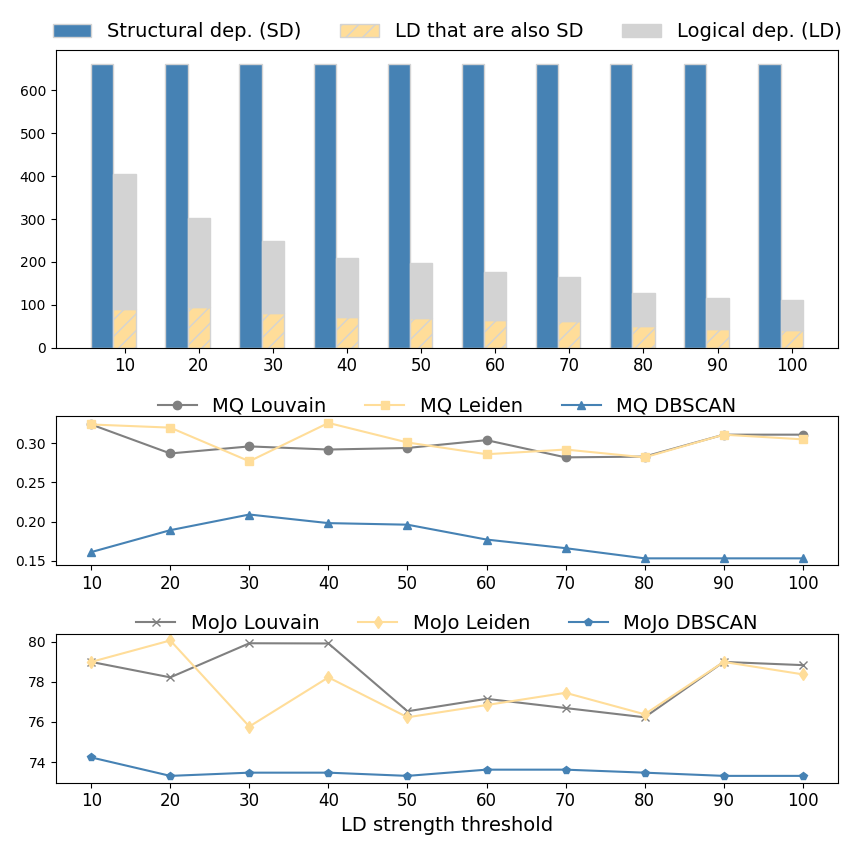
\includegraphics[width=\columnwidth]{catalina_correlation.png}
  \caption{\textbf{Apache Tomcat: Overlap between structural and logical dependencies and its correlation with clustering metrics.}}
  \label{fig:catalina_correlation}
\end{figure}

Compared with all the other systems, Apache Tomcat has the highest number of commits involved in LD extraction (Table \ref{tab:project_info}), totaling 22,698. Due to this larger information base for LD extraction, the use of logical dependencies results in better MQ values compared to other systems, as seen in Tables \ref{tab:clustering_results_ant}, \ref{tab:clustering_results_hibernate}, and \ref{tab:clustering_results_gson}.

The high number of commits leads to more effective clustering results. This highlights the importance of having a substantial commit history to enhance the quality of logical dependencies used and, consequently, the clustering solutions generated.


\subsubsection{Hibernate ORM}

\begin{figure}[t!]
  \centering
  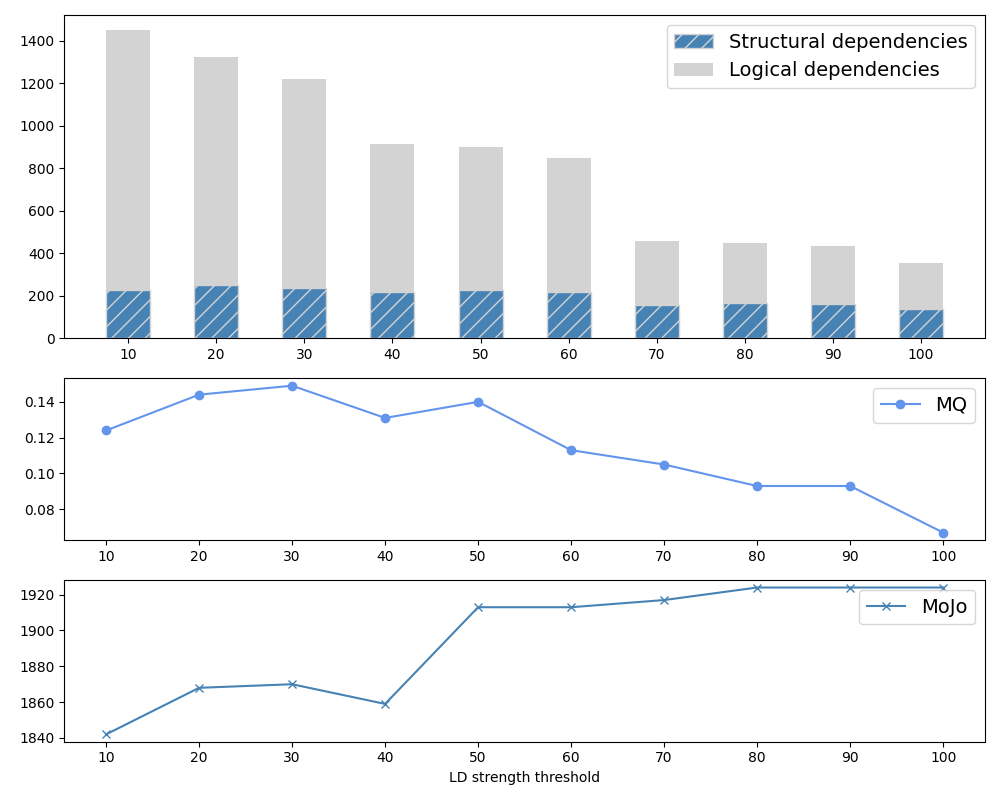
\includegraphics[width=\columnwidth]{hibernate_correlation.png}
  \caption{\textbf{Hibernate ORM: Overlap between structural and logical dependencies and its correlation with clustering metrics.}}
  \label{fig:hibernate_correlation}
\end{figure}

Hibernate ORM is the second largest in terms of the number of commits analyzed, with 16,609 commits considered for LD extraction. Additionally, it is the largest in terms of system size, with 4,414 entities (Table \ref{tab:project_info}).

Based on the results from Table \ref{tab:clustering_results_hibernate}, the SD+LD combination with a strength threshold of 30 achieved the best MQ value of 0.149 and a MoJo of 1870. The SD+LD with a strength threshold of 10 achieved the best MoJo of 1842. Similar to Apache Tomcat, the best values for both metrics are not at the same strength threshold, but even so, SD+LD[10] has a better MoJo value than SD-only.

LD-only produced the best MQ and MoJo values at 100\%, but the system coverage is again limited, with LD[100] covering only 8.07\% of the system, the lowest percentage among all systems studied. This low percentage can be connected to the number of commits compared to the number of entities. For Apache Tomcat, we had 22,698 commits and 662 entities, for Hibernate, we have 16,609 commits and 4,414 entities. This most probably means that not all entities had a chance to be updated in the versioning system.

This can also be connected to the fact that Hibernate is the only system among those studied that reaches a lower MQ value than SD-only for the SD+LD combination. Meanwhile, all other systems maintain a slightly better MQ value for SD+LD compared to SD-only, even at the highest strength threshold.


Hibernate also has the lowest overlapping percentages between LD and SD, as shown in Figure \ref{fig:hibernate_correlation}. Similar to the other systems, the MQ and MoJo performance decreases for SD+LD as the strength threshold values become stricter.

The results for Hibernate highlight the challenge of achieving better clustering in larger systems with fewer commits relative to their size.



\subsubsection{Google Gson}

Gson has the smallest number of commits analyzed, with 1,772 commits considered for LD extraction, and it is also the smallest in terms of system size, with 210 entities involved in clustering (Table \ref{tab:project_info}).

Based on the results from Table \ref{tab:clustering_results_gson}, the SD+LD combination with a strength threshold of 10 achieved the best MQ value of 0.215 and the best MoJo of 21. Similar to Apache Ant, the best values for both metrics are at the same strength threshold, and all SD+LD combinations have a better MQ value than SD-only.

LD-only produced the best MQ value at 40\%, with an MQ of 0.635 and the best MoJo value at 80\%, 90\%, and 100\%. It is the only system that produces a better result for MQ at a lower strength threshold than 100\% for LD-only. This is likely caused by the very low number of entities remaining in the system at 100\% (only 18 out of 210).

It can also be observed that Gson has the exact same metric values for MQ and MoJo for multiple strength threshold values. Again, the small number of commits and the size of the system contribute to the constant values of these metrics. This stability in the metrics suggests that smaller systems might not benefit as much from the combination of SD and LD as larger systems do.

\begin{figure}[t!]
  \centering
  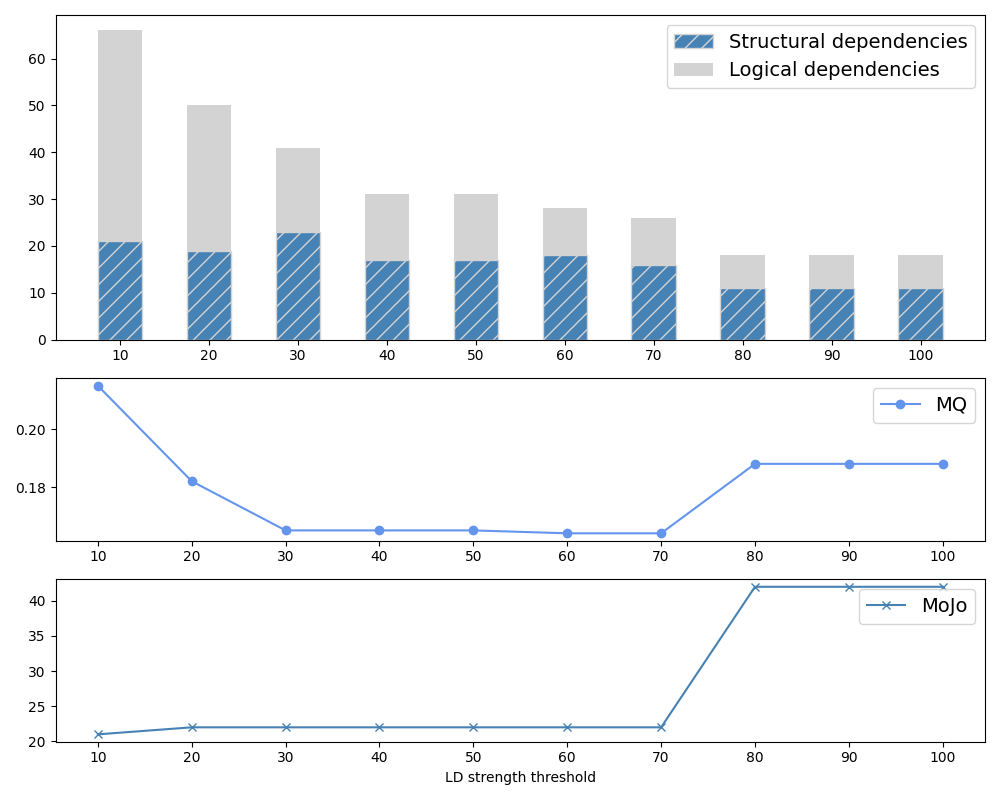
\includegraphics[width=\columnwidth]{gson_correlation.png}
  \caption{\textbf{Google Gson: Overlap between structural and logical dependencies and its correlation with clustering metrics.}}
  \label{fig:gson_correlation}
\end{figure}

Gson has relatively high overlapping rates between LD and SD compared to the other systems, as shown in Figure \ref{fig:gson_correlation}. Despite the constant values, the trend of performance decreasing with a stricter strength filtering for LD is also present for Gson.

The results for the system highlight the challenge of achieving better clustering solutions using logical dependencies in smaller systems with fewer commits. For such a small system as Gson, an improvement is still visible when using logical dependencies. However, the filtering should be done with less strict thresholds since there is a high chance of losing additional new information about the system after filtering.



\section{Conclusion}
\label{sec:conclusion}
Why did the cat get a PhD?

Because it wanted to be a purr-fessor!

\begin{thebibliography}{00}

\bibitem{b1} Ajienka, Nemitari \& Capiluppi, Andrea. (2017). Understanding the Interplay between the Logical and Structural Coupling of Software Classes. Journal of Systems and Software. 134. 10.1016/j.jss.2017.08.042.
\bibitem{b2} S. Mancoridis, B. Mitchell, C. Rorres, Y. Chen, and E. Gansner, “Using automatic clustering to produce high-level system organizations of source code,” in Proceedings. 6th International Workshop on Program Comprehension. IWPC’98 (Cat. No.98TB100242), 1998, pp. 45–52.
\bibitem{b3} V. Tzerpos and R. C. Holt, "MoJo: a distance metric for software clusterings," Sixth Working Conference on Reverse Engineering (Cat. No.PR00303), Atlanta, GA, USA, 1999, pp. 187-193, doi: 10.1109/WCRE.1999.806959.
\bibitem{b4} Stana, Adelina-Diana \& Şora, Ioana. (2023). Logical dependencies: Extraction from the versioning system and usage in key classes detection. Computer Science and Information Systems. 20. 25-25. 10.2298/CSIS220518025S. 
\bibitem{b5} Stana, Adelina-Diana \& Şora, Ioana. (2019). Analyzing information from versioning systems to detect logical dependencies in software systems. 000015-000020. 10.1109/SACI46893.2019.9111582. 
\bibitem{b6} Stana, Adelina-Diana \& Şora, Ioana. (2019). Identifying Logical Dependencies from Co-Changing Classes. 486-493. 10.5220/0007758104860493. 
\bibitem{b7} T. Zimmermann, P. Weibgerber, S. Diehl and A. Zeller, "Mining version histories to guide software changes," Proceedings. 26th International Conference on Software Engineering, Edinburgh, UK, 2004, pp. 563-572, doi: 10.1109/ICSE.2004.1317478.
\bibitem{b8} Blondel, Vincent \& Guillaume, Jean-Loup \& Lambiotte, Renaud \& Lefebvre, Etienne. (2008). Fast Unfolding of Communities in Large Networks. Journal of Statistical Mechanics Theory and Experiment. 2008. 10.1088/1742-5468/2008/10/P10008. 
\bibitem{b9} Newman, Mark. (2006). Newman MEJ.. Modularity and community structure in networks. Proc Natl Acad Sci USA 103: 8577-8582. Proceedings of the National Academy of Sciences of the United States of America. 103. 8577-82. 10.1073/pnas.0601602103. 
\bibitem{b10} S. Mancoridis, B. S. Mitchell, Y. Chen and E. R. Gansner, "Bunch: a clustering tool for the recovery and maintenance of software system structures," Proceedings IEEE International Conference on Software Maintenance - 1999 (ICSM'99). 'Software Maintenance for Business Change' (Cat. No.99CB36360), Oxford, UK, 1999, pp. 50-59, doi: 10.1109/ICSM.1999.792498.
\bibitem{b101} S. Mancoridis, B. S. Mitchell, C. Rorres, Y. Chen and E. R. Gansner, "Using automatic clustering to produce high-level system organizations of source code," Proceedings. 6th International Workshop on Program Comprehension. IWPC'98 (Cat. No.98TB100242), Ischia, Italy, 1998, pp. 45-52, doi: 10.1109/WPC.1998.693283.
\bibitem{b11} Zhihua Wen and V. Tzerpos, "An effectiveness measure for software clustering algorithms," Proceedings. 12th IEEE International Workshop on Program Comprehension, 2004., Bari, Italy, 2004, pp. 194-203, doi: 10.1109/WPC.2004.1311061.
\bibitem{b12} Şora, Ioana. (2013). Software Architecture Reconstruction through Clustering: Finding the Right Similarity Factors. 45-54. 10.5220/0004599600450054. 
\bibitem{b13} A. Corazza, S. Di Martino, V. Maggio and G. Scanniello, "Investigating the use of lexical information for software system clustering," 2011 15th European Conference on Software Maintenance and Reengineering, Oldenburg, Germany, 2011, pp. 35-44, doi: 10.1109/CSMR.2011.8.
\bibitem{b14} Anquetil, Nicolas \& Lethbridge, Timothy. (1998). File Clustering Using Naming Conventions for Legacy Systems. 10.1145/782010.782012. 
\bibitem{b15} Oliva, Gustavo \& Gerosa, Marco Aurelio. (2012). A Method for the Identification of Logical Dependencies. Proceedings - 2012 IEEE 7th International Conference on Global Software Engineering Workshops, ICGSEW 2012. 70-72. 10.1109/ICGSEW.2012.19. 
\bibitem{b16} Silva, Luciana \& Valente, Marco \& Maia, Marcelo. (2015). Co-change Clusters: Extraction and Application on Assessing Software Modularity. Transactions on Aspect-Oriented Software Development. 10.1007/978-3-662-46734-3\_3. 
\bibitem{b17} Murtagh, Fionn \& Contreras, Pedro. (2012). Algorithms for hierarchical clustering: An overview. Wiley Interdisc. Rew.: Data Mining and Knowledge Discovery. 2. 86-97. 10.1002/widm.53. 
\bibitem{b18} Amarjeet Prajapati, Anshu Parashar, Amit Rathee. Multi-dimensional information-driven many-objective software remodularization approach. Frontiers of Computer Science in China, 17(3):173209, 2023.


\end{thebibliography}

\begin{IEEEbiographynophoto}{First} Add text here
\end{IEEEbiographynophoto}

\begin{IEEEbiographynophoto}{Second} Add text here
\end{IEEEbiographynophoto}

\EOD

\end{document}
